\documentclass[11pt,ngerman,a4paper]{article}
%Gummi|061|=)
\usepackage{amsmath}
\usepackage{a4wide}
\usepackage{amsthm}
\usepackage{amsbsy}
\usepackage[separate-uncertainty=true]{siunitx}
\usepackage{booktabs}
\usepackage{amssymb}
\usepackage{inputenc}
\usepackage{rotating} 
\usepackage{graphicx}
\usepackage{paralist}
\usepackage{selinput}
\SelectInputMappings{%
adieresis={ä},
germandbls={ß},
}

\title{\textbf{Versuch V102: Drehschwingungen}}
\author{Martin Bieker\\
		Julian Surmann\\
		\\
		Durchgef\"{u}hrt am 23.01.2013\\
		TU Dortmund}
\date{}
\usepackage{graphicx}
\begin{document}
\renewcommand\tablename{Tabelle}
\renewcommand\figurename{Abbildung}
\maketitle
\thispagestyle{empty}
\newpage
\clearpage
\setcounter{page}{1}

\section{Einleitung}
Der folgende Versuch behandelt Drehschwingungen. Dabei wird ein Metalldraht, an dem eine Masse hängt, ausgelenkt und so in periodische Schwingungen versetzt.Im ersten Versuchsteil werden die elastischen Konstanten untersucht. Bei diesen handelt es sich um Proportionalitätsfaktoren zwischen den relativen Verformungen und den pro Fläche angreifenden Flächen.
Im zweiten Versuchsteil wird (auch mit Drehschwingungen) das magnetische Moment eines Permanentmagneten in der Kugel bestimmt.
\section{Theorie}
In der Physik gibt es zwei Arten von Kräften, die auf Festkörper wirken: Entweder, die Kräfte wirken auf jedes Volumenelement (z.B. die Schwerkraft), oder sie wirken nur auf die Körperoberfläche. Erstere sind in der Lage, eine Änderung des Bewegungszustandes zu bewirken. Letztere können nur Volumens- oder Gestaltsänderungen erzeugen und spielen in diesem Versuch die entscheidende Rolle. Die sogenannte Spannung beschreibt die Oberflächenkraft pro Fläche. Diese kann in eine Normalspannung und eine Tangentialspannung aufgeteilt werden. Ist die Spannung hinreichend klein, sind die auftretenden Längen- oder Volumenänderungen proportional zu diesen Anteilen:
\begin{equation}
\label{1}
\sigma = E\frac{\Delta L}{L}
\end{equation}
\begin{equation}
\label{2}
P = Q\frac{\Delta V}{V}.
\end{equation}
Dieser Zusammenhang heißt Hook'sches Gesetz.\newline
In diesem Versuch wird das elastische Verhalten von isotropen Körpern betrachtet. Das heisst, dass die elastischen Konstanten richtungsunabhängig sind. Zwei Konstanten reichen dann aus, um das elastische Verhalten vollständig zu beschreiben. Es existieren viel elastische Konstanten:
\begin{itemize}
\item Torsionsmodul G: Beschreibt die Gestaltselastizität.
\item Kompressionsmodul Q: Beschreibt die Volumenelastizität.
\item Elastizitätsmodul E: Beschreibt die relative Längenänderung des Körpers in Richtung der angreifenden Normalspannung.
\item Poissonsche Querkontraktionszahl $\mu$: Beschreibt die relative Längenänderung des Körpers senkrecht zu der angreifenden Normalspannung.
\end{itemize}
Zwischen ihnen gilt folgender Zusammenhang:
\begin{equation}
E = 2G(\mu+1)=3Q(1-2\mu)
\label{3}
\end{equation}
\subsection{Torsionsmodul}
Das Schubmodul G beschreibt die Gestaltelastizität eines Körpers. Wenn nur Tangentialspannungen angreifen, treten Gestaltsänderungen auf. Um eine Scherung handelt es sich, wenn die parallelen Ebenen ihre Form beibehalten und um einen bestimmten Betrag verschoben werden. Dieser Betrag wächst proportional mit dem Abstand zur Grundfläche. Dies ist in Abbildung \ref{?} zu erkennen.
Es gilt
\begin{equation}
\label{4}
G = \frac{\tau}{\alpha}.
\end{equation}
Zur Bestimmung des Torsionsmoduls G wird hier die dynamische Methode verwendet. Dazu wird ein Metalldraht, an dem unten eine Kugel mit einem Trägheitsmoment $\theta$ befestigt ist. Das obere Ende des Drahtes ist fest eingespannt. Dieses System führt nach einer Auslenkung Drehschwingungen aus. Die Schwingungen sind ungedämpft, da an der Kugel zwei entgegengesetzte Drehmomente angreifen.
Dann gilt für die Schwingungsdauer T
\begin{equation}
\label{5}
T=2\pi \sqrt{\frac{\theta}{D}}.
\end{equation}
Die Richtgröße D des Zylinders ist mit
\begin{equation}
\label{6}
D=\frac{\pi  R^4 G}{2L}
\end{equation}
Aus diesen Gleichungen bildet sich also das Torsionsmodul mit
\begin{equation}
\label{8}
G=\frac{8\pi\theta L}{R^4T^2}.
\end{equation}
gegeben. Das Trägheitsmoment einer Kugel (mit Aufhängung) beträgt
\begin{equation}
\label{7}
\theta=\frac{2R_k^2m_k}{5}+\theta_K.
\end{equation}

\subsection{Magnetisches Moment}
Das magnetische Moment
\begin{equation}
\label{9}
\vec{m}=p\vec{a} 
\end{equation}
ist ein Maß für die Stärke eines magnetischen Dipols. Wird nun ein Magnet in ein homogenes Magnetfeld mit der Flussdichte $\vec{B}$  gebracht, wirkt auf ihn ein Drehmoment, dass mit
\begin{equation}
\label{10}
\vec{M_{Mag}}=\vec{m} \times \vec{B} = m B sin(\gamma)
\end{equation}
Dabei soll $\gamma$ der Winkel zwischen den Feldlinien und der Geraden, die durch die magnetischen Pole geht, sein.
Die Schwingungsdauer mit Magnet beträgt dann
\begin{equation}
\label{11}
T_m=2\pi \sqrt{\frac{\theta}{mB+D}}.
\end{equation}
Für den Betrag des magnetischen Feldes innerhalb eines Helmholzspulenpaar gilt der folgende Zusammenhang:
\begin{equation}
B = \mu_0 \frac{8\,I}{\sqrt{125}\,R} 
\label{helm}
\end{equation}
\section{Aufbau}

Die in diesem Versuch verwendete Messapparatur ist den Abbildungen ??? und ??? zu entnehmen. Ein Metalldraht (Torsionsdraht) ist mit seinem oberen Ende fest an einem Stativ befestigt. An dem Draht hängt eine Metallkugel. Am Torsionsdraht ist ein kleiner Spiegel befestigt. Das Licht einer Glühlampe wird mit einem Spalt und einer Sammellinse gebündelt und so angebracht, dass es den Spiegel bescheint. Der sich um die Hochachse drehende Spiegel beleuchtet nun bei einem spezifischen Winkel eine Photodiode, die mit einer elektrischen Schaltung eine Stoppuhr auslöst. So kann die Schwingungsdauer gemessen werden.
\subsection{Elektrische Schaltung zur Messung der Periodendauer}
Um die Periodendauer zu messen, wird der analoge Widerstand der Photodiode in ein digitales Signal (d.h. Hell/Dunkel) umgewandelt. Bei einem Übergang von High nach Low wird dann der Takteingang eines Flopflops geschaltet. Der Ausgang des Flipflops wird direkt in die Stoppuhr gespeist. Es ist zu beachten, dass zur Messung der Periodendauer drei Lichtsignale benötigt werden. Dies ist an Abbildung ???[die zweite] gut zu erkennen. Daher eignet sich der Takteingang der Flopflops, dieser schaltet beim ersten Lichtsignal auf Low, die Stoppuhr wird aktiviert. Beim zweiten Lichtsignal wird lediglich der Ausgang des Flipflops auf High geschaltet. Auf die Uhr hat das keinen Einfluss, da diese lediglich von Übergängen von High auf Low schaltet. Beim dritten Lichtsignal wird die Uhr dann gestoppt, genau zum Ende einer Periodendauer. Aus Gründen der Einfachheit wird die Stoppuhr manuell zurückgesetzt.
\section{Durchführung}
\subsection{Messung des Torsionsmodules}
Nachdem die Schaltung aufgebaut ist und die Messapparatur genügend ausgerichtet ist (Lichtstrahl und Spiegel), wird der Torsionsdraht ausgelenkt und mehrere Werte für die Periodendauer aufgenommen.
\subsection{Messung des magnetischen Moments}
Die Durchführung zur Messung des magnetischen Moments ist ähnlich zu 4.1, allerdings wird jetzt der Magnet in der Metallkugel waagerecht ausgerichtet und mit Hilfe einer um die Kugel aufgebauten Helmholzspulen-Paar ein Magnetfeld erzeugt. Auch hier werden mit Hilfe der Schaltung mehrere Werte für die Schwingungsdauer aufgezeichnet.
\section{Auswertung}

\subsection{Bestimmung des Schubmoduls}
Zunächst muss das Trägheitsmoment der Kugel bestimmt werden. Der hierfür benötigte Radius und die Masse der Kugel, sowie das Trägheitsmoment der Kugelhalterung wurden am Versuchsaufbau abgelesen und so auf
\begin{itemize}
\item $m_K = \SI{0,5122+-0,0002}{\kilo\gram}$
\item $R_K =\SI{0.0253800+-0.0000018}{\metre}$
\item $\theta_K = \SI{22.5e-7}{\kilo\gram\meter\squared}$
\end{itemize}
bestimmt. Hieraus kann das Gesamträgheitsmoment der Kugel mit Aufhängung nach Formel 8 berechnet werden. Es ergibt sich ein Wert von
\[
\theta = \SI{0.00013422+-0.00000005}{\kilo\gram\meter\squared}
\]
Die gemessenen Werte für die Periodendauer befinden sich in Tabelle 1. Hieraus werden Mittelwert und Standardabweichung bestimmt:
\[
\overline{T} = \SI{18.4600+-0.0021}{\second}
\]
Aus diesen Werten ergibt sich für das Schubmodul ein Wert von
\[
G = \SI{9.5+-2.1e+10}{\newton\per\meter\squared}.
\]

\subsection{Bestimmung des magnetischen Moments}

Zur Bestimmung des magnetischen Moments eines Permamagneten im Innern der Kugel, wurde die Schwingungsdauer der Aperatur einem externen Magnetfeld gemessen. Die Mittelwerte von $T$ in Abhängigkeit von Strom $I$ in der Felderzeugenden Spule sind in Tabelle 2 dargestellt. Die Stärke des durch ein Helmholzspulenpaar erzeugten Magnetfeldes ist durch Formel 12 gegeben. Trägt man den Kehrwert des gemessenen Periodendauer zum Quadrat gegen das Magnetfeld auf, ergibt sich wegen Formel 11
\begin{equation}
\frac1{T^2}= \frac{m}{4\pi^2\theta}\cdot B + \frac{D}{4\pi^2\theta} 
\end{equation}
ein linearer Zusammenhang (siehe Abb. \ref{ausw}).
\begin{figure}[h]
\centering
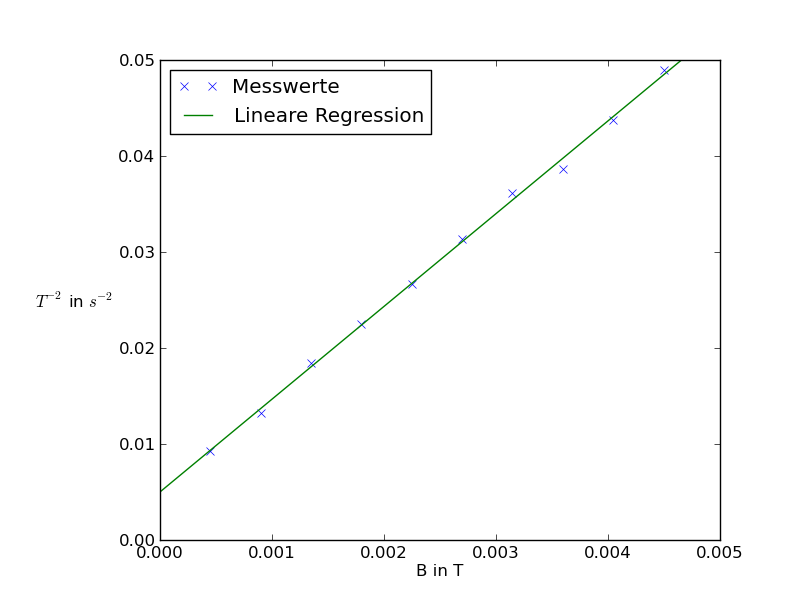
\includegraphics[scale=0.7]{Abb4.png}
\caption{$\frac1{T^2}$ in Abhängigkeit von der magnetischen Feldstärke}
\label{ausw}
\end{figure}
 Eine lineare Ausgleichsrechnung ergibt für die Steigung der Geraden 
\[
\frac{m}{4\pi^2\theta} = \num{9.56+-0.12}\,.
\]
Hieraus folgt für das magnetische Moment:
\[
m = \SI{0.0506+-0.0006}{\ampere\meter\squared}.
\]
\subsection{Bestimmung der Stärke des Erdmagnetfelds}
Um die Stärke des Erdmagnefeldes zu bestimmen, wird der Permamagnet in der Kugel parallel zu diesem, d.h. senkrecht zur Drehachse, ausgerichtet. Der Mittelwert der gemessenen Schwinungsdauer beträgt
\[
\overline{T^*} = \SI{18.887+-0.032}{\second}\,.
\]
Stellt man Formel 11 nach $B$ um
\begin{equation}
B = \frac{\frac{\theta}{4\pi^2T^2}-D}{m}
\end{equation}
kann mit den bereits bestimmten Werten für $\theta$, $D$ (Formel 6) und $m$ der Betrag das Erdmagnetfeldes berechnet werden. Dieser beträgt
\[
B_{Erde} = \SI{0.000303+-0.000004}{\tesla}\,.
\]
\section{Diskussion}

\section{Literatur- und Abbildungsverzeichnis}
\begin{itemize}
\item $[1]$: Der Praktikumsanleitung zu V354 der TU Dortmund entnommen. Download am 5.1.14 unter \newline http://129.217.224.2/HOMEPAGE/PHYSIKER/BACHELOR/AP/SKRIPT/V354.pdf
\end{itemize}
\section{Anhang}
\begin{itemize}
\item Tabellen und Abbildungen
\item Auszug aus dem Messheft.


\end{itemize}

\newpage
\begin{table}[H]
\centering
\begin{tabular}{|c|lllllll|}
\hline
&18.474&18.471&18.473&18.473&18.463&18.466&18.466\\
$\frac{T}{\si{\second}}$ &18.462 & 18.469& 18.460&  18.460 & 18.454&18.459&18.453\\&18.457&18.435&18.457&18.453&18.457&18.447&18.450\\
\hline
\end{tabular}

\caption{Periodendauer $T$ bei der Messung ohne magnetische Einflüsse}
\end{table}
\begin{table}
\centering
\begin{tabular}{lll}
\toprule
{$\frac{I}{\si{\ampere}}$} &{ $\frac{B}{\si{\tesla}}$} &{ $\frac{T}{\si{\second}}$ }\\
\midrule
0.1 & 0.00045 & $10.3840 \pm 0.0060$ \\
0.2 & 0.000899 & $8.6870 \pm 0.0060$ \\
0.3 & 0.001349 & $7.3580 \pm 0.0040$ \\
0.4 & 0.001798 & $6.6682 \pm 0.0021$ \\
0.5 & 0.002248 & $6.1200 \pm 0.0019$ \\
0.6 & 0.002698 & $5.6454 \pm 0.0023$ \\
0.7 & 0.003147 & $5.2630 \pm 0.0070$ \\
0.8 & 0.003597 & $5.0860 \pm 0.0060$ \\
0.9 & 0.004046 & $4.7800 \pm 0.0040$ \\
1.0 & 0.004496 & $4.5216 \pm 0.0022$ \\
\bottomrule
\end{tabular}
\label{}
\caption{Periodendauer $T$ in Abhängigkeit von der magnetischen Feldstärke}
\end{table}
\end{document}
